\chapter{Experimental Procedures}

\section{Preparation of the Studied (6,5)-enriched Single-Wall Carbon Nanotube (SWCNT) Dispersion }

\subsection{Synthesis of SWCNTs}

Catalytic chemical vapor deposition (CCVD) is a standard method for synthesizing carbon nanotubes (CNTs) \cite{prasek2011methods, agboola2007conceptual}. This technique depends on the decomposition of carbon sources, such as methane and acetylene, via heat or plasma irradiation to form carbon nanotubes on a substrate \cite{agboola2007conceptual}. Such reactions are typically driven by transition-metal catalysts such as nickel, iron, and cobalt \cite{prasek2011methods}.

One commonly used process known as the CoMoCAT method involves catalytic reactions that include cobalt (Co) and molybdenum (Mo) as catalysts \cite{resasco2002scalable}. Here, carbon monoxide gas (CO) is used as a carbon source that decomposes in the reaction 
\vspace{-2mm}
\begin{equation}
\ce{CO_(g) + CO_{(g)} $\rightarrow$ CO_{2(g)} + C_{(CNT)}},
\end{equation}
to form carbon nanotubes \cite{resasco2002scalable}. This process is typically conducted at temperatures between 700 - \SI{900}{\celsius} and pressures ranging from 1 - 10 atm \cite{resasco2002scalable}. To date, all carbon nanotube growth methods only produce an ensemble of nanotubes with varying chiralities. As such, these ensembles are often used as precursor materials for filtration techniques capable of creating dispersions that are enriched by a single chirality \cite{ichinose2017extraction, liu2011large}.

\subsection{Dispersion of SWCNTs}
We created a (6,5)-enriched dispersion sample by starting with CoMoCAT SWCNTs obtained from Sigma-Aldrich (Manufacturer Number: Signis$^{\tiny{\textregistered}}$ SG65i). This initial product consists of a powder of SWCNTs with an average diameter of 0.78 nm and a median length of \SI{1}{\micro \meter}. Approximately 95\% of the SWCNTs are semiconducting with 41\% of them being (6,5) SWCNTs . In this powdered form, SWCNTs have a tendency to form ropes and bundles due to strong van der Waals interactions as high as \SI{500}{\electronvolt / \micro \meter} between nanotubes \cite{vaisman2006role}. 

\begin{figure}[h]
	\centering
	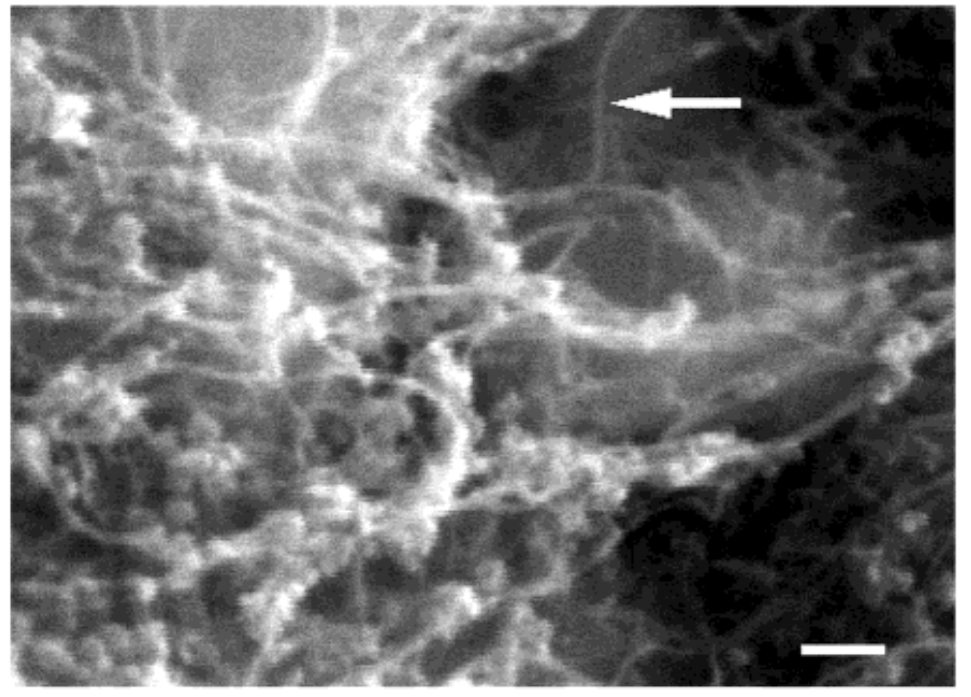
\includegraphics[scale=0.3]{images/chapter_methods/sem_cnt_powder_bandy}
	\caption{(a) Scanning electron microscope image of nanotube powder. The scale bar corresponds to 200 nm. The arrow indicates a single rope emerging out of the nanotube bundle. Reproduced from Ref.\ \cite{bandyopadhyaya2002stabilization}.}
\end{figure}

%Objective is to create a (6,5)-enriched sample. Variety of chiralities leads to several peaks in optical spectrum. We want to be able to create enriched sample by %removing chiralities that are not of interest. Hard to do this when carbon nanotubes of various chiralties bundle together. Cannot do any filtration methods to %selectively remove certain chiralities. Hence, we disperse the CoMoCAT SWCNTS in an aqueous solution to as a first step towards creating a (6,5)-enriched sample. 

First, we disperse CoMoCAT SWCNTs in an aqueous solution containing surfactants by using sonication followed by ultracentrifugation \cite{ichinose2017extraction}. Sonication uses mechanical vibrations to break up the van der Waals interactions occuring in nanotube bundles \cite{tkalya2012use}. Furthermore, the presence of surfactants, such as sodium dodecyl sulfate (SDS), has the effect of mitigating inter-tube interactions to stabilize the suspension by preventing the formation of nanotube bundles \cite{vaisman2006role}. In the aqeuous dispersion, SDS molecules become adsorbed on the outer surface of the nanotubes as shown in Figure \ref{fig:sds_molecule}. Here, the hydrophobic part of SDS becomes adsorbed onto the nanotube surface while the hydrophilic part points towards the aqueous phase and aids with the dissolution of the nanotube \cite{richard2003supramolecular}. This forms a distribution of negative charge on nanotube surfaces due to the negatively-charged hydrophilic region that, via Coulomb interactions, prevents nanotubes from sustaining physical contact \cite{richard2003supramolecular}. 

\begin{figure}[h]
\centering
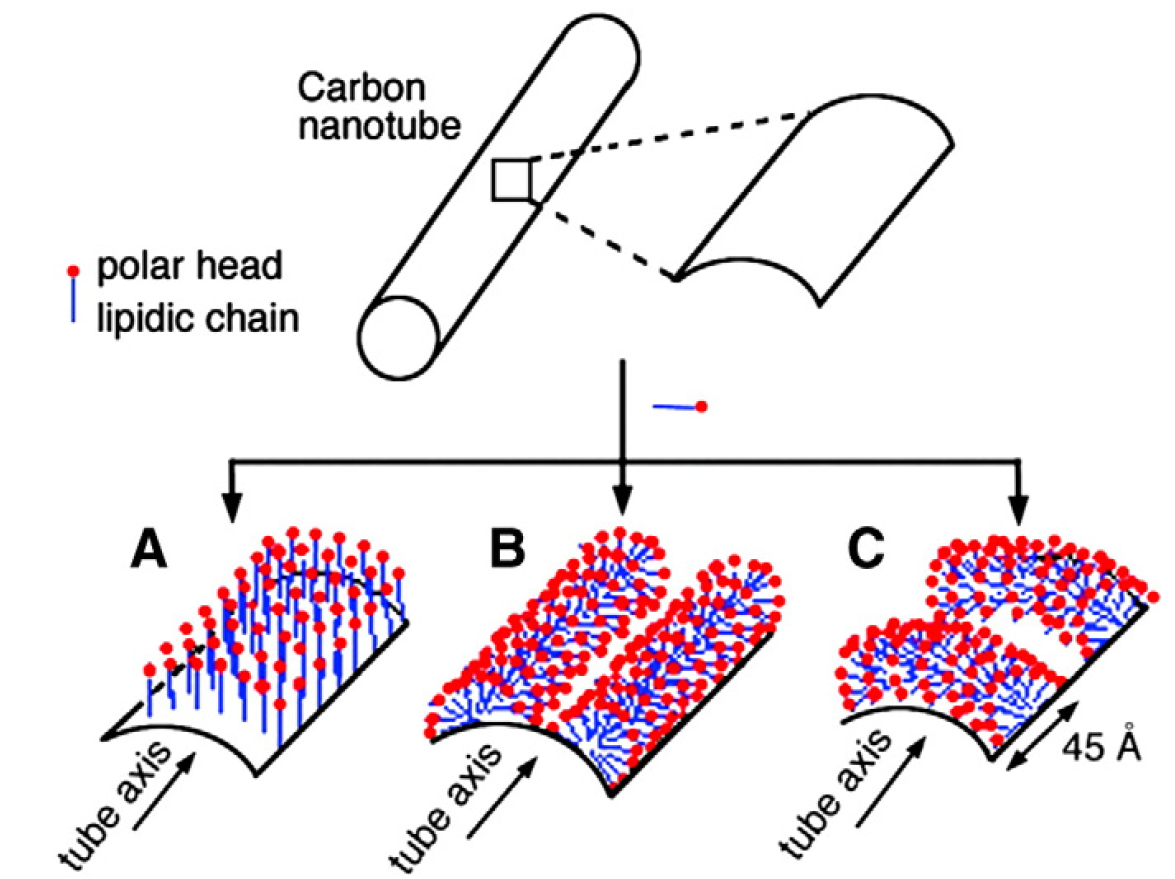
\includegraphics[scale=0.3]{images/chapter_methods/surfactant_tkalya}
\caption{Surfactants such as sodium dodecl sulfate (SDS) can become adsorbed on the surfaces of SWCNTs in three ways. (A) Adsorbed SDS molecules form a monolayer on the nanotube surface. In addition, adsorbed SDS molecules can form half-cylinders on the surface of nanotubes that are (B) aligned parallel to the tube axis or (C) aligned perpendicular to the tube axis. Reproduced from Ref.\ \cite{richard2003supramolecular}. }	
\label{fig:sds_molecule}
\end{figure}

Unfortunately, not all nanotube bundles can be broken up by sonication. Therefore, ultracentrifugation is used to separate dispersed nanotubes from the remaining bundles. This yields a mixture composed of nanotubes floating in the aqeuous solution above a sediment of nanotube bundles. We then extract the aqeuous solution containing the dispersed nanotubes, also known as the supernatant, and perform gel chromatography on this product to obtain a (6,5)-enriched sample.

Gel chromatography works by separating CNTs according to their relative diameters \cite{ichinose2017extraction}. which include sodium dodecyl sulfate (SDS) and sodium cholate (SC) with concentrations of 0.5\% each, using sonication followed by ultracentrifugation. CNTs dispersed in aqueous solutin placed in a column containing hydrogel beads at the bottom. Adjusting pH of aqueous solution affects adsorption of nanotubes onto the beads. At starting pH, metallic nanotubes come out first. Then as pH is lowered, can now elute semiconducting SWCNTs followed by smaller diamter SWCNTs. 



In this process, the presence of a small concentration (4\%) of sodium deoxycholate (DOC), a surfactant, in the dispersion prevents nanotubes from clumping together to form bundles. Finally, the sample is pipetted into a quartz cuvette with an optical path length of 1 mm. 

%Include figure of absorption spectrum
\subsection{Optical Spectrum of (6,5)-enriched Sample}

Measuring the absorbance of prepared samples provides a means of determining the different chiralities present in the sample as well as their relative populations. Here, absorbance $A$ is defined as 
\begin{equation}
A = \log_{10}\left(\dfrac{I_{\mathrm{ref}}}{I_{\mathrm{sample}}}\right),
\end{equation}
where $I_{\mathrm{ref}}$ and $I_{\mathrm{sample}}$ represent the optical transmission through a reference sample and the nanotube sample respectively. The reference sample only contains water and a 4\% concentration of DOC and is also stored in a cuvette with an optical path length of 1 mm. 

Figure \ref{fig:sample_absorbance} presents the absorbance spectrum of the (6,5) sample measured using the white-light supercontinuum source described in Section \ref{section:white_light_probe}. The spectrum exhibits a number of optical transitions including the $E_{11}$, phonon sideband, $E_{12}$, and $E_{22}$ resonances at photon energies of 1.26, 1.45, 1.9, and 2.17 eV respectively. Furthermore, other small peaks in the sample at 1.35 and 1.41 eV emerge from exciton resonances of (9,1) and (6,4) nanotubes respectively.

\begin{figure}[H]
	\centering
	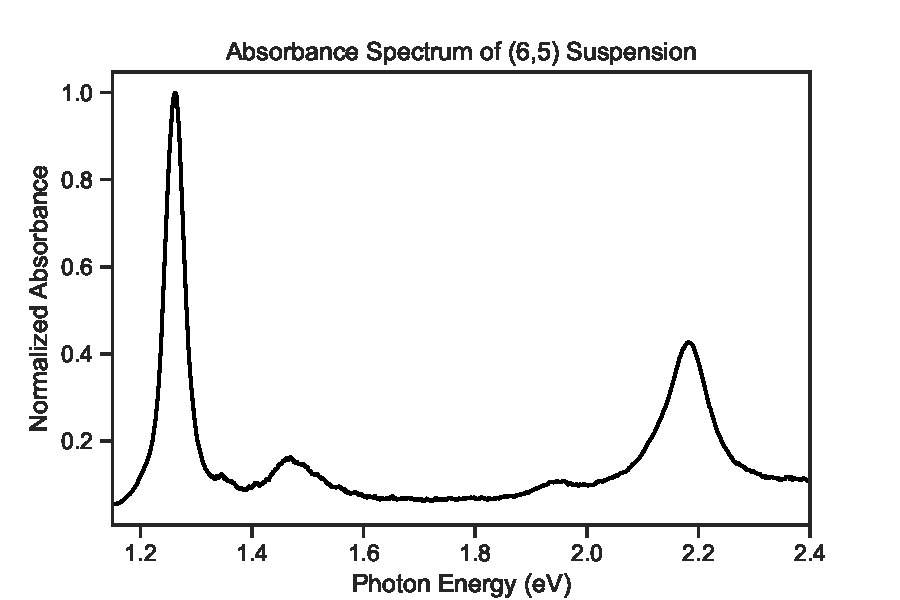
\includegraphics[scale=0.7]{images/chapter_methods/sample_absorbance}
	\caption{ Absorbance spectrum of (6,5) sample.}
	\label{fig:sample_absorbance}
\end{figure}

\section{Experimental Apparatus for Pump-Probe Spectroscopy}

%include figure of setup
\subsection{Overview}
The experimental apparatus, illustrated in Figure \ref{fig:setup_schematic}, incorporates the use of an intense optical pump pulse followed by a broadband probe pulse to characterize the ultrafast carrier dynamics of carbon nanotubes. The pump and probe beams are focused onto surface of the sample in a non-collinear geometry. Finally, the transmission spectrum of the probe is resolved using a spectrometer to resolve the non-equilibrium optical properties of the sample.  


\begin{figure}[h]
	\centering
	\includegraphics[scale=0.7]{example-image-a}
	\caption{ Schematic Diagram of the Experimental Apparatus. }
	\label{fig:setup_schematic}
\end{figure}


\subsection{Chirped Pulse Amplifier and Optical Parametric Amplifier}
The CPA-2010 laser source manufactured by Clark-MXR functions as the heart of this optical setup. This laser generates amplified pulses using a chirped pulse amplification process. It operates at a repetition rate of 1 KHz and outputs pulses with a 150 fs duration, a central wavelength of 775 nm, and a pulse energy of 1 mJ. Finally, the CPA-2010 serves as a pump laser for the optical parametric amplifier (OPA). 

The OPA used in the setup is a TOPAS-800 produced by Light Conversion. \cite{topas}. It emits signal and idler beams via a superfluoresence in a barium borate (BBO) crystal which are then amplified in four subsequent stages. The signal and idler wavelengths span 1.1 - 1.5 $\mu$m  and 1.5 - 2.7 $\mu$m respectively. Furthermore, an additional BBO crystal placed at the output of the OPA provides a means of generating the second harmonic of the signal or idler which can be used an optical pump.

\subsection{Filters}

The setup features a wavelength separator that seperates the fundamental of the signal (FS) from the second harmonic of the signal (SHS). This optical device contains a set of two dichroic mirrors that reflect the SHS and transmit the FS. As a result of the second harmonic generation process, the polarization of SHS remains perpendicular to that of FS. Hence, a half-wave plate is placed in the optical path of the SHS and appropriately adjusted to make the polarizations of FS and SHS parallel to each other. 

In addition to this, two neutral density wheels are used to attenuate the intensity of the probe and the optical pump.

\subsection{White Light Continuum Probe}


\label{section:white_light_probe}
Supercontinuum generation represents a nonlinear optical process by which the spectrum of an incident laser pulse becomes significantly broadened \cite{dubietis2017ultrafast}. It has been observed to occur in many different media such as water, fused silica, sapphire and calcium fluoride \cite{dubietis2017ultrafast}. This process is facilitated by the formation of a filament which starts as a result of self-focusing \cite{dubietis2017ultrafast}. In other words, the refractive index of the supercontinuum generation medium depends on the intensity of propagating light \cite{dubietis2017ultrafast}. Due to the interplay between this self-focusing and other competing effects such as self-phase modulation, and multiphoton absorption, the spectrum  broadens as the pulse travels through the medium \cite{dubietis2017ultrafast}. 

In this setup, supercontinuum generation occurs by focusing the fundamental of the signal beam (FS) into a sapphire crystal with a thickness of 5 mm. Here, the center of the sapphire crystal is placed at a distance of one focal length of the lens used to focus the FS. This process generates a white-light continuum that spans 1 - 2.4 eV. 

Finally, an iris is placed in path of FS such that its aperture is positioned at the center of the FS beam. This iris is used to crop the outer portion of the FS, thereby reducing its the beam diameter. Doing this has been observed to have the effect of minimizing the temporal fluctuations of the generated white light spectrum. 

\subsection{Motorized Delay Stage and Optical Shutter}

The setup includes a motorized delay stage and an optical shutter that are used to control the pump conditions in each measurement.

The delay stage consists of a pair retro-reflecting mirrors mounted on a motorized stage. The pump beam travels to both of these mirrors. Hence, adjusting the position of the motorized stage alters the time delay between the pump and probe pulses by either increasing or decreasing the optical path length traveled by the pump pulse. 

The optical shutter makes it possible block the pump beam in order to measure probe transmission through the sample under equilibrium conditions. At each time delay, the transmission of the probe beam is measured with the pump beam blocked and with the pump beam unblocked by the shutter. Conducting measurements in this manner mitigates the effect of long-term fluctuations in the laser output. 

\subsection{Spectrometer}
The probe is collected into an optical fibre which sends the probe beam to a (\textbf{\color{red} NAME OF SPECTROMETER}) spectrometer built by Princeton Instruments.  The spectrometer uses a grating with a diffraction grating with a blaze wavelength of 800 nm and a groove density of (\textbf{\color{red} ADD GROOVE DENSITY}) per mm. The diffracted light is then imaged onto a CCD camera to measure the probe spectrum. 

The camera is silicon-based and contains an array of 1340 $\times$ 100 pixels. Finally, the camera must be cryogenically cooled to \SI{-100}{\celsius} using liquid nitrogen for an optimal signal-to-noise ratio.


\subsection{Pump and Probe Spot Sizes}
The pump and probe spot sizes are measured using a knife edge scan technique \cite{firester1977knife}. For this, a razor blade attached to a post is mounted on a motorized stage placed in the sample position. The sharp edge of the blade faces in a direction perpendicular to that of the direction of propagation of the incident beam. A power meter is placed behind the razor blade to measure the average power of the transmitted beams.

As the motorized stage moves the razor blade's position laterally with respect to the beam's propagation direction, the razor blade increasingly blocks portions of the incident beam.  Measuring the transmitted power of incident beam as a function of the razor blade position yields a cumulative distribution function of the incident light's intensity.

\begin{figure}[h]
	\centering
	\includegraphics[scale=0.7]{example-image-a}
	\caption{Example measurement of beam diameter for pump and probe. Solid lines are fits to the data using function defined in equation}
	\label{fig:beam_diamter_measurement}
\end{figure}

Assuming that the beam diameter can be approximated as a Gaussian distribution, the spot size can be estimated by fitting this data with the equation 
\begin{equation}
	P = P_0 + \dfrac{P_{\mathrm{max}}}{2} \left( 1 - \mathrm{erf} \left( \dfrac{\sqrt{2}(x - x_0)}{w} \right) \right),
\end{equation}
which represents the cumulative distribution function of a Gaussian distribution. This function yields the beam diameter $w$. Furthermore, $P_0$ represents the baseline of the power meter observed when the beam is fully blocked, erf stands for the standard error function, $P_{max}$ denotes the maximum power of the beam, $x$ parametrizes the position of the blade and $x_0$ indicates the position at which the blade blocks 50\% of the incident beam's average power.  







